\documentclass[11pt,a4paper]{article}
\usepackage[latin1]{inputenc}
\usepackage[margin=1in]{geometry}
\usepackage{amsmath}
\usepackage{amsfonts}
\usepackage{amssymb}
\usepackage{graphicx}
\setlength\abovedisplayskip{0pt}
\author{James Brissette}
\title{CS-6350: HW 2}
\begin{document}
	\maketitle
	
	\section{Linear Classifiers and Boolean Functions}
		\begin{enumerate}
			\item $\neg x_1 \vee x_2 \vee \neg x_3 $: Linearly separable $\rightarrow (1-x_1)+x_2 + (1-x_3) \geq 1$
			\item $(x_1 \vee x_2) \wedge x_3$: Linearly separable $\rightarrow \frac{1}{2}(x_1 + x_2) + x_3 \geq 1.5$
			\item $(x_1 \wedge \neg x_2) \vee \neg x_3$: Linearly separable $\rightarrow \frac{1}{2}(x_1 + (1-x_2))+(1-x_3) \geq 1$
			\item $x_1$ xor $x_2$ xor $x_3$: Not linearly separable.
			\item $x_1 \wedge \neg x_2 \wedge x_3$: Linearly separable $\rightarrow x_1 + (1-x_2) + x_3 \geq 3$
		\end{enumerate}
	
	\section{Feature transformations}
		\begin{enumerate}
			\item My function is $\phi ( x_{1} , x_{2} ) = ( x_{1}^{4} , x_{2}^{3} )$, which maps $x_{1}$ and $x_{2}$ to $x_{1}^{4}$ and $x_{2}^{3}$ respectively. And in this space the function is linearly separable as $$\phi(fr(x_1,x_2)) = \begin{cases}
			+1 \quad 17x_1+16x_2 \leq r \\
			-1 \quad otherwise
			\end{cases}$$
			\item We can see that since the original function $17x_1^4-16x_2^3$ was $\leq r$, it follows the linear classifier for the new function is equivalent to $-w^T\phi (x_1,x_2) \geq b$
		\end{enumerate}
	
	\section{Mistake Bound Model of Learning}
		\begin{enumerate}
			\item $ $
			\begin{enumerate}
				\item Since the concept class C consists of one function for every combination of $z$, which is $\{0,1\}^n$, $\vert C_1 \vert = 2^n$ 
				\item The algorithm would proceed as follows:\\
				\textit{\textbf{Observe example \\
				predict 0\\
				if correct, no update, continue\\
				if incorrect, learning ends as the  target function has been learned.}}\\ \\
				Since there is only one target function, and given that the function only evaluates to 1 for one single instance of the sample space (when x = z), there will never be a mistake so long as the learner continues to predict 0. When the learner finally encounters $z$, it will update and can continue to progress with the assurance that since $z$ has been found, there will never be another mistake. 
			\end{enumerate}
			\item $ $
			\begin{enumerate}
				\item If we assume in the worst case that nature is adversarial, then the CON algorithm will make $n-1$ mistakes. Because there are $n$ function where $f_i(x) = x_i$. Suppose our target function is $f_n$ and out randomly drawn function was $f_1$, we would then have a mistake, and proceed to randomly choose from $C - \{f_1\}$. This would continue $n-1$ times until at last the last function left in $C$ to evaluate was the target function $f$.
				\item Since the halving algorithm predicts the majority label, $f_i$ would predict with the majority on every example except $x_i$, and would be correct every time. The majority will always predict 0 and will not incur any mistakes since there is in fact only one correct function. The only mistake will occur when $f_i$ predicts 0 with the majority on example $x_i$ when in fact it is correct. At that point the halving algorithm will eliminate all functions $f\in C$ which are not consistent, a set containing ONLY $f_i$, and learning ends after one mistake.
			\end{enumerate}
		\end{enumerate}
	
	\section{The Perceptron Algorithm and its Variants}
		\begin{enumerate}
			\item I used python3 to implement the Perceptron algorithm variants. I chose not to represent the data in a full 19-dimensional vector given how sparse the data is (imagine there were 100 dimensions). Instead I used an array of dictionaries where each entry in the array corresponds to a row item in the data, and each item is itself a dictionary whose key-value pairs correspond to the attributes and respective values. For examples, if the entry were to read: +1 3:15 4:29 13:30 .. the dictionary structure would appear: \{label: 1, 3:15, 4:29, 13:30\}. This implementation didn't allow me to leverage numpys vector library, but the additional overhead involved in looping was minimal and is more memory efficient. In terms of evaluating each of the variants, I chose to create a cross validation function to handle identifying the best hyper-parameters, one dedicated function for each variant, as well as one test function for each to evaluate the best parameter combinations on the test set.
			\item Given the most frequent label in the training set (+1), the accuracy on the development set is .56, and the test set is .525
			\item Noting that the random initialization may sometimes give different results with respect to the best hyper-parameters, in most cases I ran the 5-fold cross validation (for ten epochs each) several times and averaged them to see, on average, which parameters were \textit{actually} the best (however, the below results are based on a single random instance of the algorithm on the data). My results were as follows:\\ \\
			\textbf{Simple Perceptron}    \\
			a) rate = \{.01\}  \\
			b) cross-validation accuracy using rate=.01 was \textbf{0.612733}\\
			c) total number of updates on the training set was \textbf{6015}\\
			d) the best accuracy on the development set came with using 16 epochs and yielded an accuracy of \textbf{.735} (see below for the plot used to determine the best epoch to use). This yielded a weight vector, bias combination as follows:\\
			\begin{gather}
				w = [-4.790801  , -6.310801  , 18.629199  ,  0.809199  , -9.290801,\\
				-8.960801  , -3.480801  ,  1.899199  ,  0.75067916, -1.05087573,\\
				0.91483852,  1.0267039 ,  3.30614975,  1.8007971 ,  0.88184558,\\
				0.41990239, -2.7867524 , -0.66128905, -2.170801  ] \\
				b = -4.567802999999947
			\end{gather}
			e) using the weight vector and bias from epoch 16 to predict on the test set, the algorithm reported an accuracy of \textbf{.587065} \\
			f)
			\begin{center}
				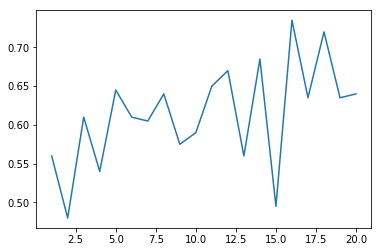
\includegraphics[width=0.7\linewidth]{simple_plot}
			\end{center}
			~\\
			\textbf{Decaying Perceptron}    \\
			a) For the specific combination of the random shuffling of the training data and the initial weight vector and bias, I found the optimal initial rate = \{1\}  \\
			b) cross-validation accuracy using rate=1 was \textbf{0.664533}\\
			c) total number of updates on the training set was \textbf{5113}\\
			d) the best accuracy on the development set came with using 17 epochs and yielded an accuracy of \textbf{.71} (see below for the plot used to determine the best epoch to use). This yielded a weight vector, bias combination as follows:\\
			\begin{gather}
			w = [-0.52830582, -0.62562476,  4.58366762,  1.83460061, -0.48774808,\\
			-2.43257835, -2.71244112, -1.11330101,  0.85833871, -1.40136228,\\
			-2.3033998 , -1.70711248,  0.57267534,  0.43230634,  0.20699507,\\
			0.06603351, -0.31253566, -0.08022425, -0.59702606] \\
			b = -32.005986
			\end{gather}
			e) using the weight vector and bias from epoch 17 to predict on the test set, the algorithm reported an accuracy of \textbf{.71144} \\
			f)
			\begin{center}
				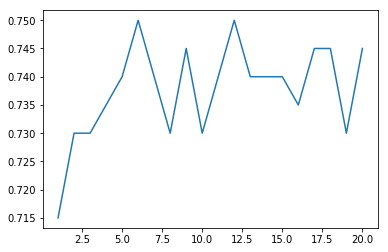
\includegraphics[width=0.7\linewidth]{decaying_plot}
			\end{center}
			~\\
			\textbf{Margin Perceptron}    \\
			a) For the specific combination of the random shuffling of the training data and the initial weight vector and bias, I found the optimal combination of hyper-parameters to be margin=.01, rate=1  \\
			b) cross-validation accuracy using margin=.01, rate=1 was \textbf{0.6880}\\
			c) total number of updates on the training set was \textbf{4930}\\
			d) the best accuracy on the development set came with using 14 epochs and yielded an accuracy of \textbf{.6} (see below for the plot used to determine the best epoch to use). This yielded a weight vector, bias combination as follows:\\
			\begin{gather}
			w = [-0.54624921, -0.95548707,  2.26801139,  0.52011042, -1.45902761,\\
			-1.02471788,  0.10777735, -0.68208914, -0.01616318, -0.57514031,\\
			0.97513725,  0.30675042,  0.21458043,  0.21317788,  0.17914802,\\
			0.07836919, -0.30403893, -0.05202941,  0.01070719] \\
			b = -1.008271999999998
			\end{gather}
			e) using the weight vector and bias from epoch 14 to predict on the test set, the algorithm reported an accuracy of \textbf{.721393} \\
			f)
			\begin{center}
				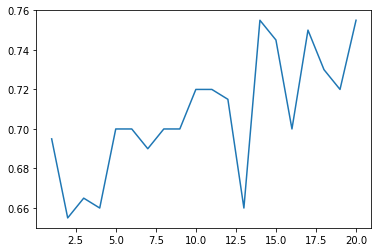
\includegraphics[width=0.7\linewidth]{margin_plot}
			\end{center}
			~\\
			\textbf{Averaged Perceptron}    \\
			a) For the specific combination of the random shuffling of the training data and the initial weight vector and bias, I found the optimal initialization of the hyper-parameter to be rate=.01  \\
			b) cross-validation accuracy using rate=.01 was \textbf{0.6840}\\
			c) total number of updates on the training set was \textbf{5959}\\
			d) the best accuracy on the development set came with using 12 epochs and yielded an accuracy of \textbf{.735} (see below for the plot used to determine the best epoch to use). This yielded an averaged weight vector and bias combination as follows:\\
			\begin{gather}
			avg_w = [-39297.52976   , -49249.90396   , 180277.36      ,  25541.91      ,\\
         -71399.98      , -91189.06      , -56378.89      ,   1073.7       ,\\
           5291.2546671 , -28886.41068276,  16675.62511214,  12328.1483673 ,\\
          21168.53398624,   8564.77647009,   3173.97610439,   1201.88086327,\\
         -22542.91907643,  -5259.25862048,  -5631.41756   ] \\
			avg_b = 4.559999999999947
			\end{gather}
			e) using the weight vector and bias from epoch 12 to predict on the test set, the algorithm reported an accuracy of \textbf{.726368} \\
			f)
			\begin{center}
				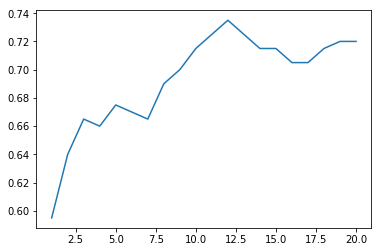
\includegraphics[width=0.7\linewidth]{average_plot}
			\end{center}
			~\\
			\textbf{Aggressive Perceptron}    \\
			a) For the specific combination of the random shuffling of the training data and the initial weight vector and bias, I found the optimal initialization of the hyper-parameter to be margin=.1  \\
			b) cross-validation accuracy using margin=.1 was \textbf{0.6667}\\
			c) total number of updates on the training set was \textbf{450}\\
			d) the best accuracy on the development set came with using 16 epochs and yielded an accuracy of \textbf{.75} (see below for the plot used to determine the best epoch to use). This yielded an averaged weight vector and bias combination as follows:\\
			\begin{gather}
			w = [-0.00364741, -0.02665061,  0.03840352,  0.00146818, -0.02537675,\\
         -0.01593747,  0.0012163 , -0.00015176, -0.00049352, -0.00296716,\\
         -0.0025369 ,  0.00382602,  0.00923817,  0.00805557,  0.00699792,\\
          0.00613048, -0.00274205,  0.00251772, -0.01891303]\\
			b = 4.559999999999947
			\end{gather}
			e) using the weight vector and bias from epoch 16 to predict on the test set, the algorithm reported an accuracy of \textbf{.791045} (This initially seemed high to me considering the other algorithms, so I ran it a few more times to estimate the average accuracy and indeed noticed the probability of this level of accuracy is very low, though this is indeed what the result was!)\\
			f)
			\begin{center}
				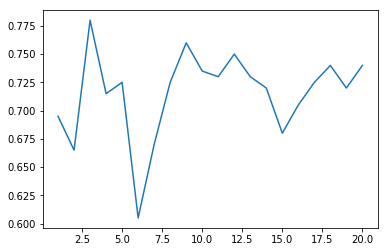
\includegraphics[width=0.7\linewidth]{aggressive_plot}
			\end{center}
		\end{enumerate}
	
\end{document}